\section{Технологическая часть}

\subsection{Выбор технологических средств}
В качестве языка программирования был выбран Python, поскольку он предоставляет множество необходимых для реализации поставленной задачи библиотек, такие как aiohttp, socket, bencodepy и прочие, а также ввиду имеющего опыта работы с этим языком. 

Была выбрана среда разработки PyCharm, поскольку она бесплатна для студентов и хороша знакома, так как активно использовалась в процессе обучения.

Для создания удобного, интуитивно понятного интерфейса использовался набор библиотек PyQt5. \newline

\subsection{UML диаграмма классов}
На Рисунках \ref{fig300:image}-\ref{fig301:image} приведена UML-диаграмма основных разработанных классов. На диаграмме \ref{fig301:image} приведены все виды сообщений, которыми могут обмениваться участники процесса скачивания.

\begin{figure}[h]
	\begin{center}
		{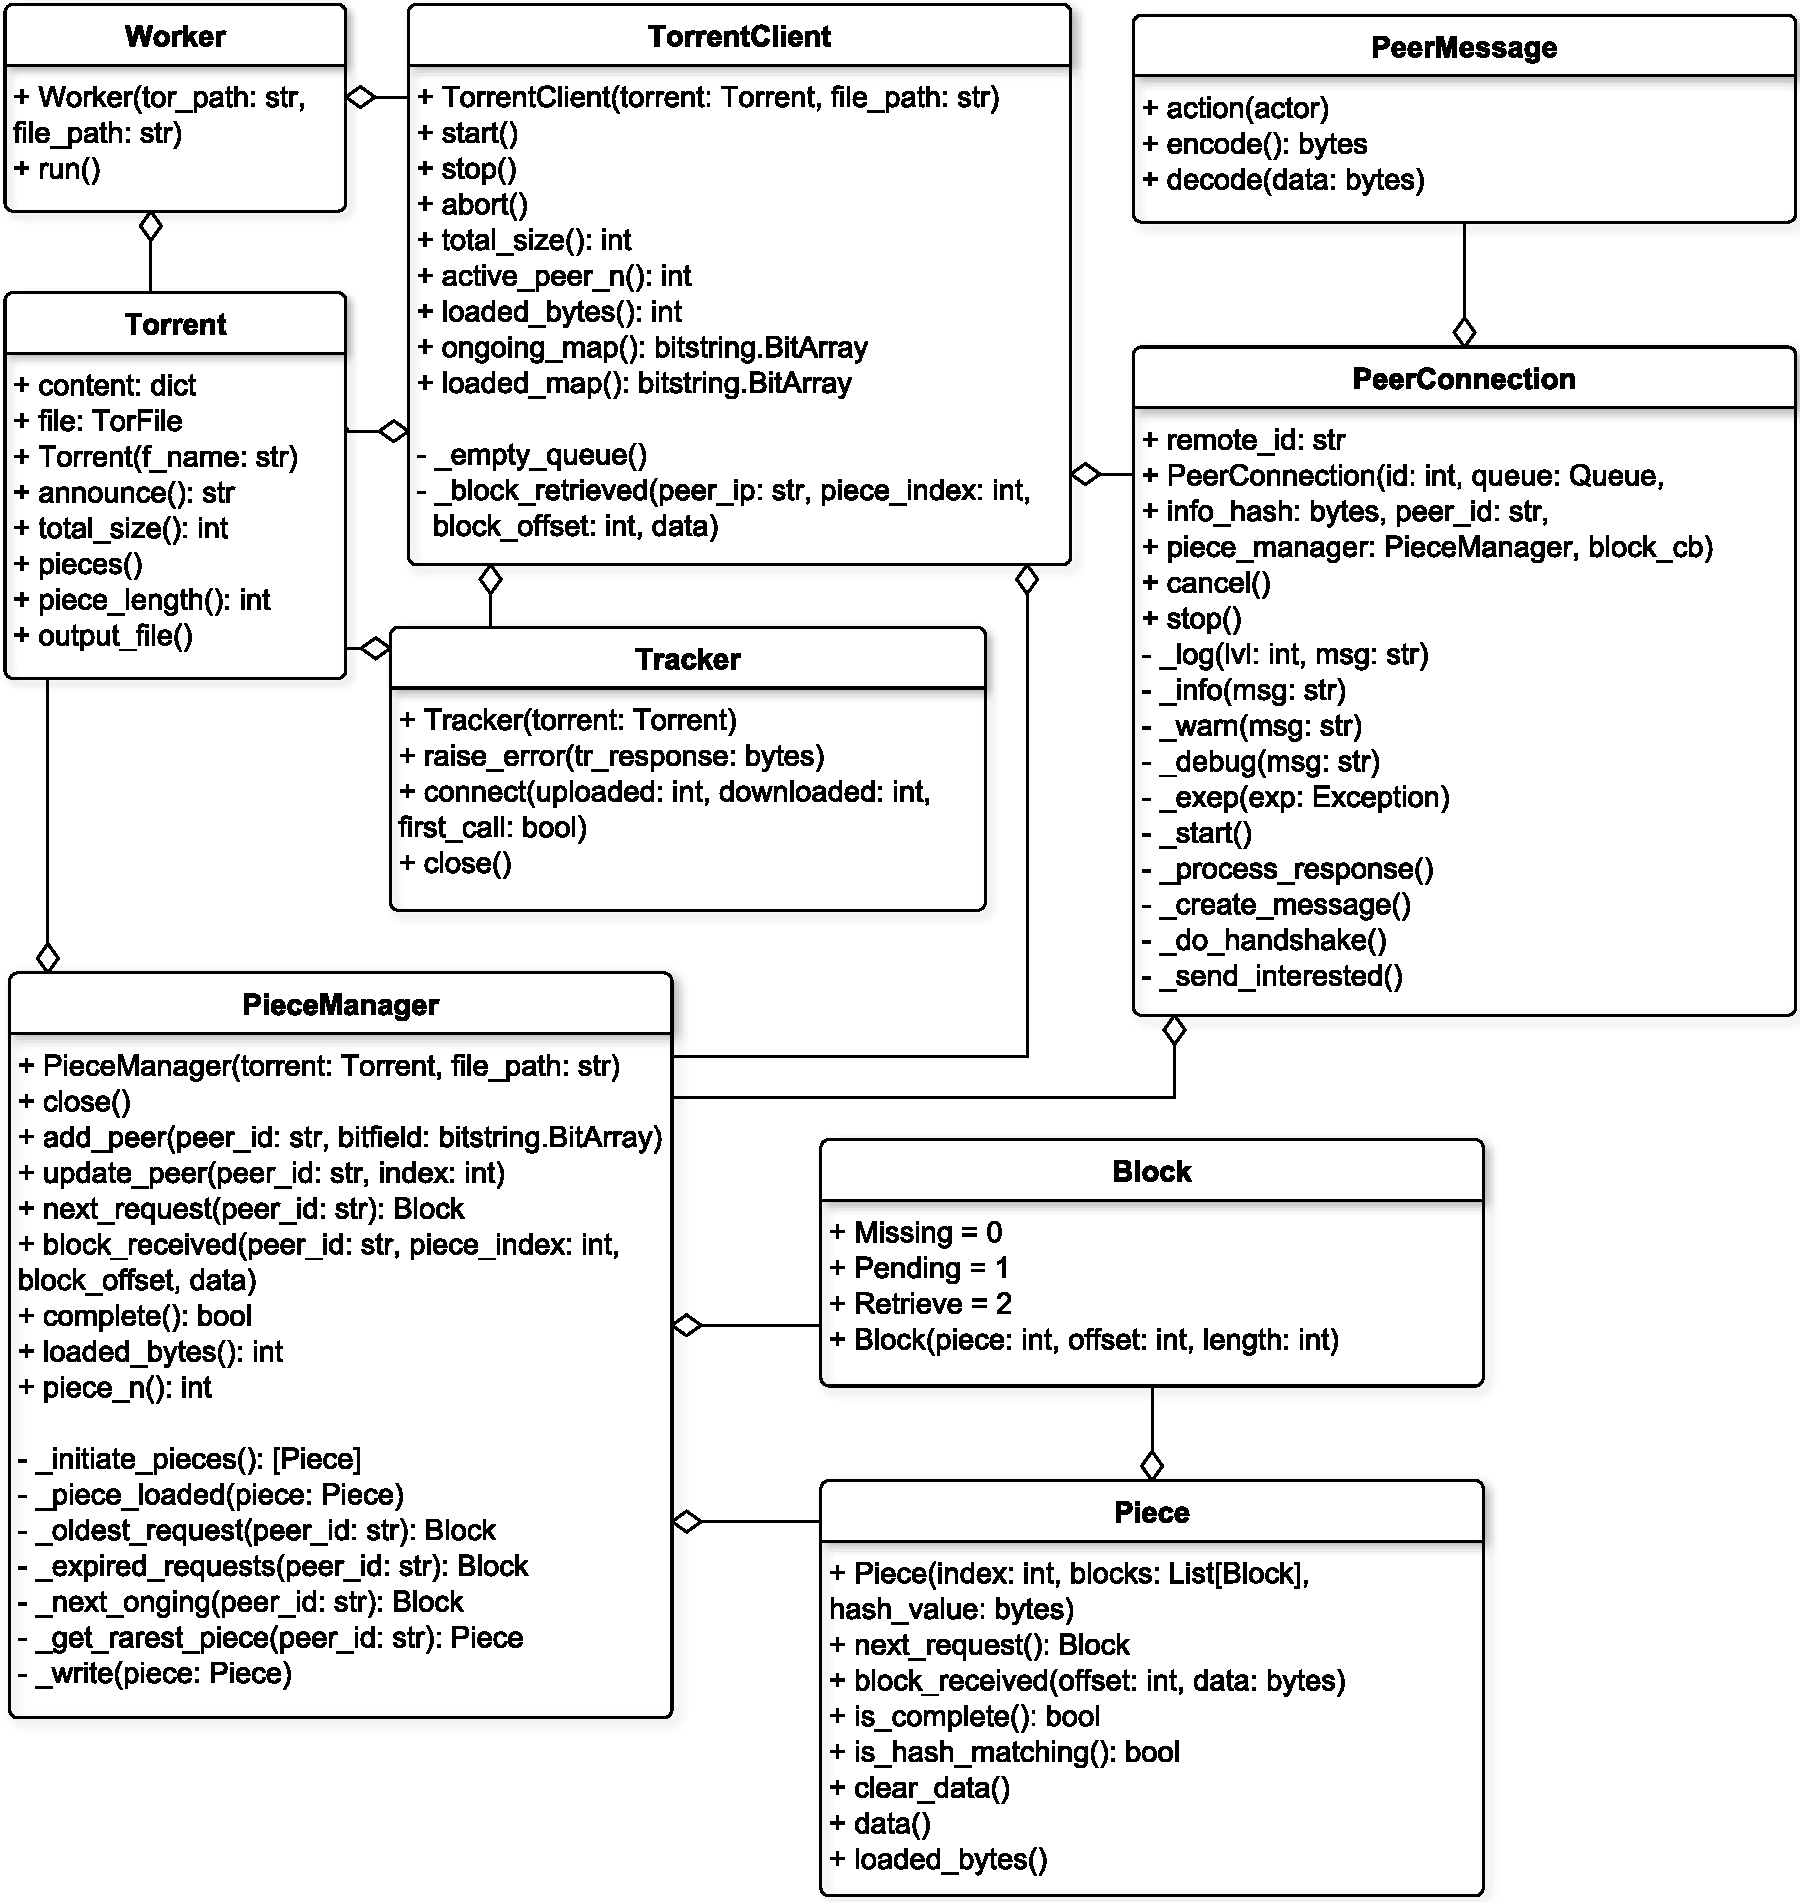
\includegraphics[scale = 0.57]{img/uml.pdf}}
		\caption{UML-диаграмма классов}
		\label{fig300:image}
	\end{center}
\end{figure}

\begin{figure}[h]
	\begin{center}
		{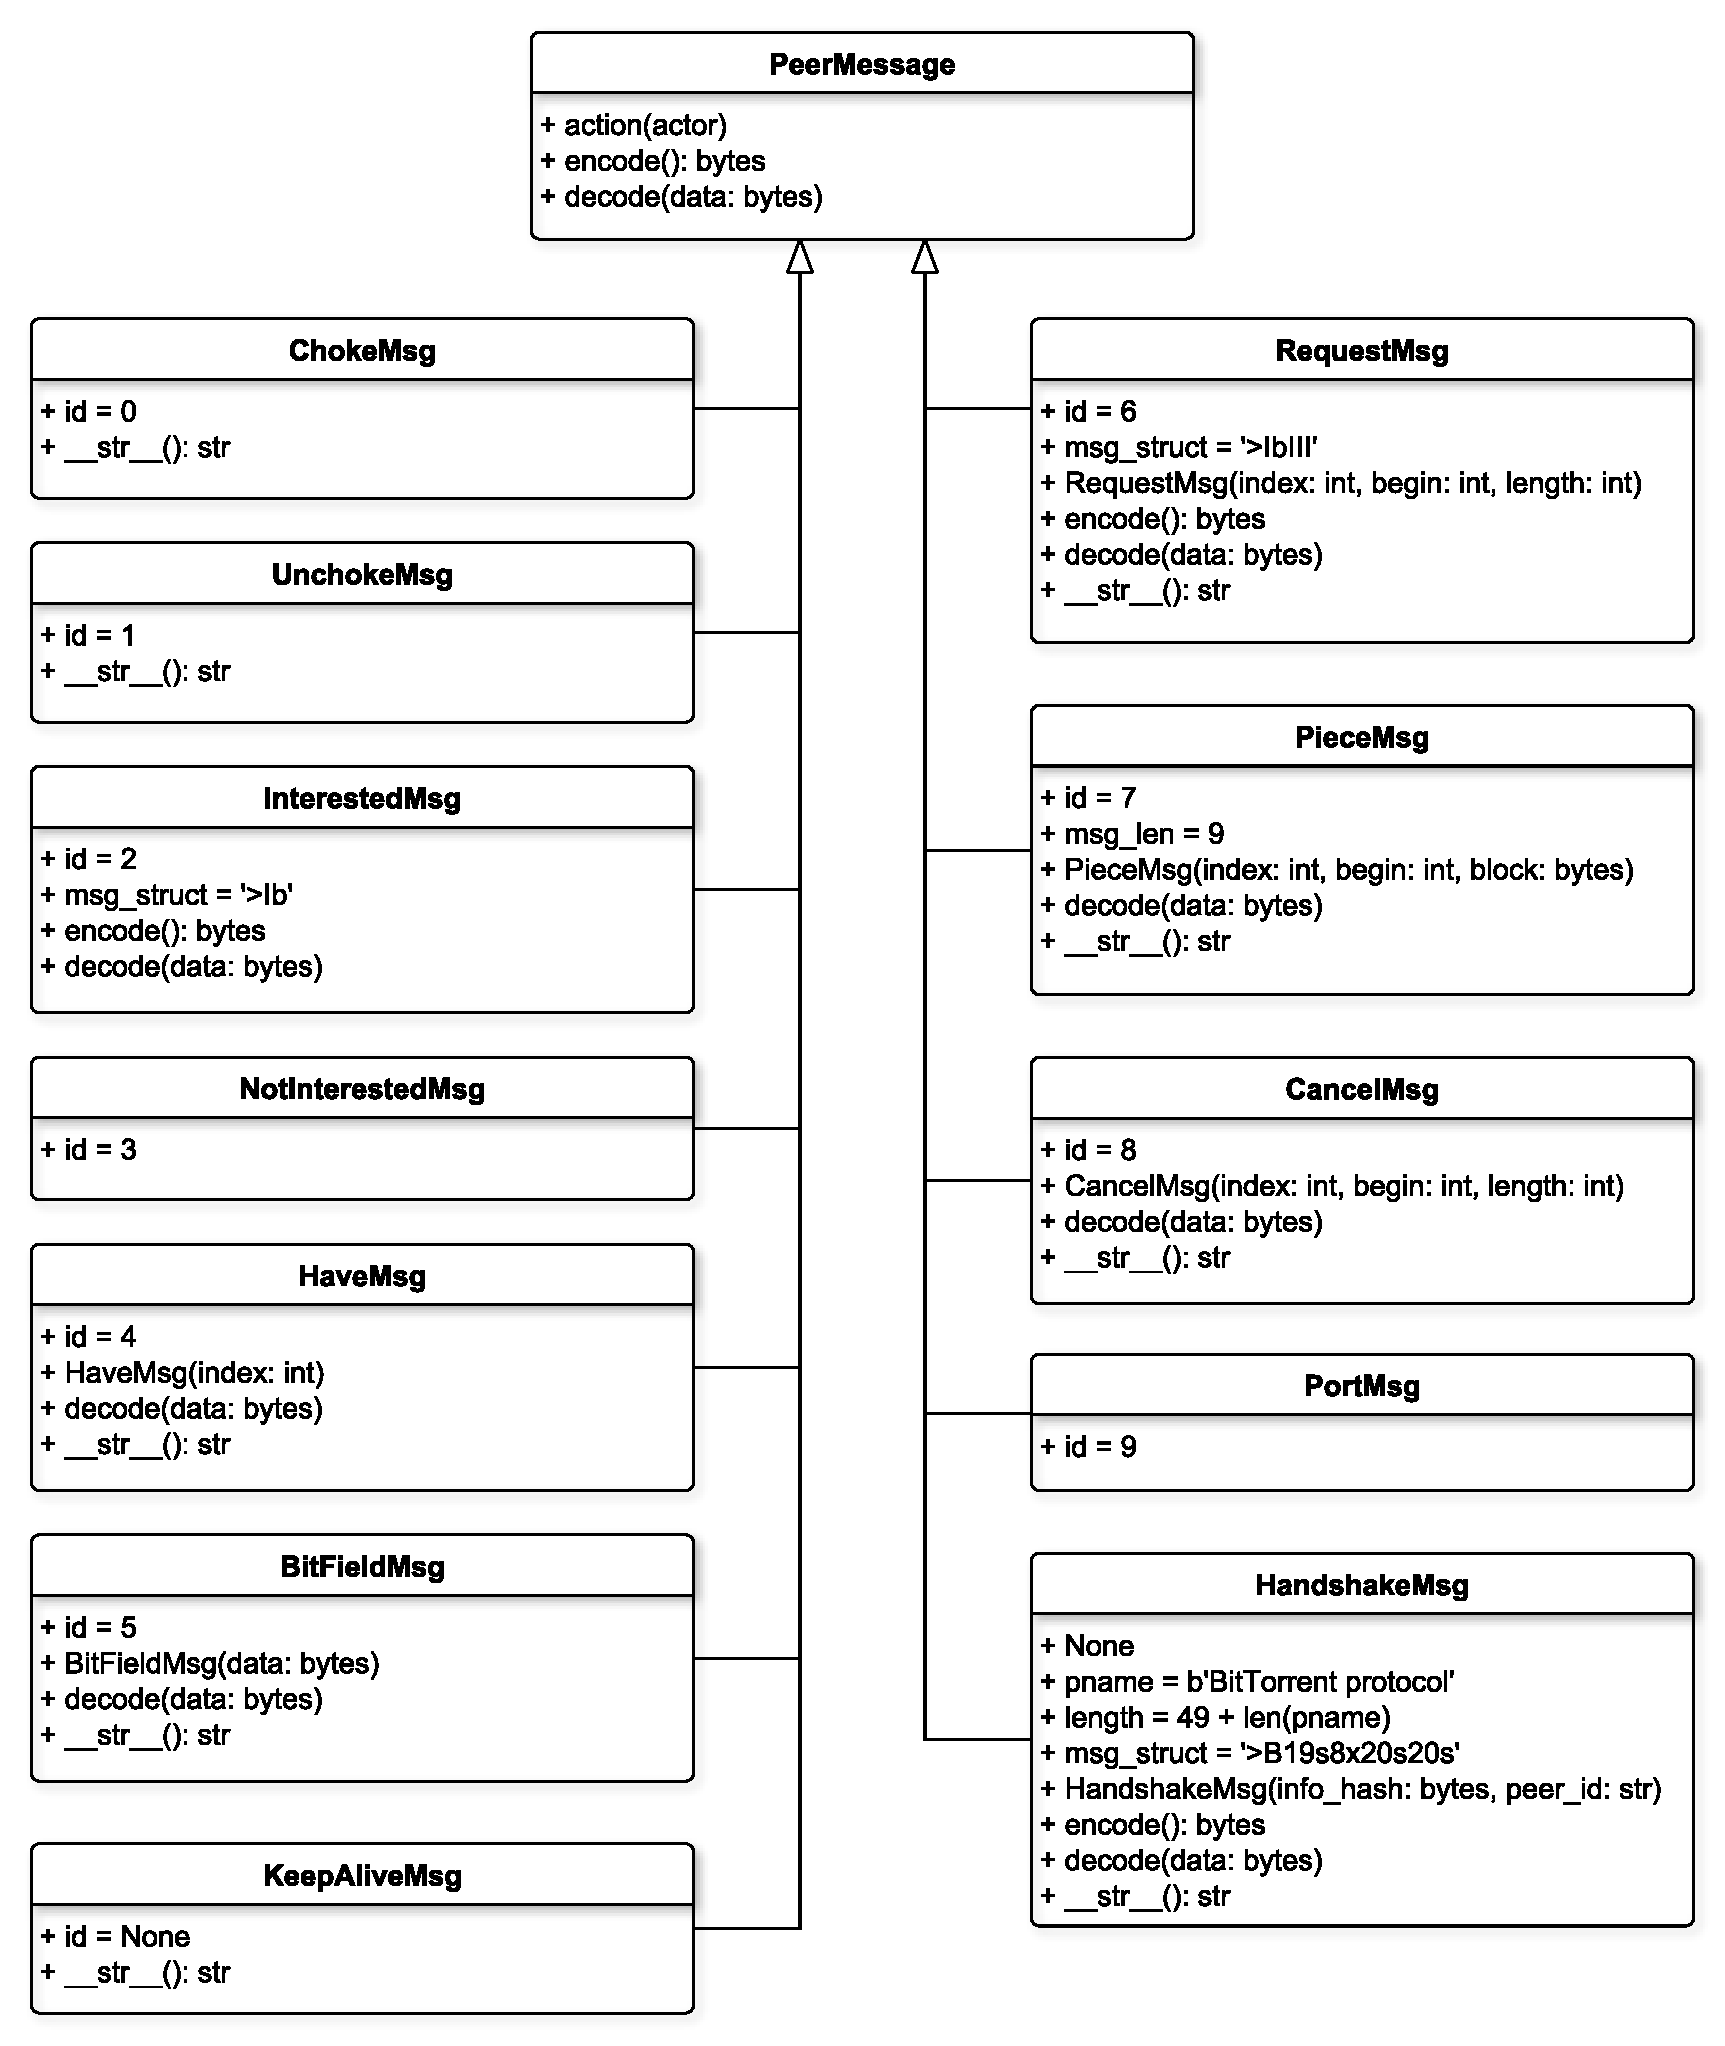
\includegraphics[scale = 0.57]{img/msgs.pdf}}
		\caption{UML-диаграмма классов сообщений}
		\label{fig301:image}
	\end{center}
\end{figure}